\documentclass[14pt]{article}
\usepackage[a4paper, margin=2cm]{geometry}
\usepackage{graphicx}

\title{Introduction to \latex\ 2}
\author{Tasriad Ahmed Tias}
\date{\today}

\begin{document}
    \maketitle

    \tableofcontents
    \listoffigures
    \pagebreak
    \section{Inserting image}
    \subsection{include graphics}
    image1:\newline
    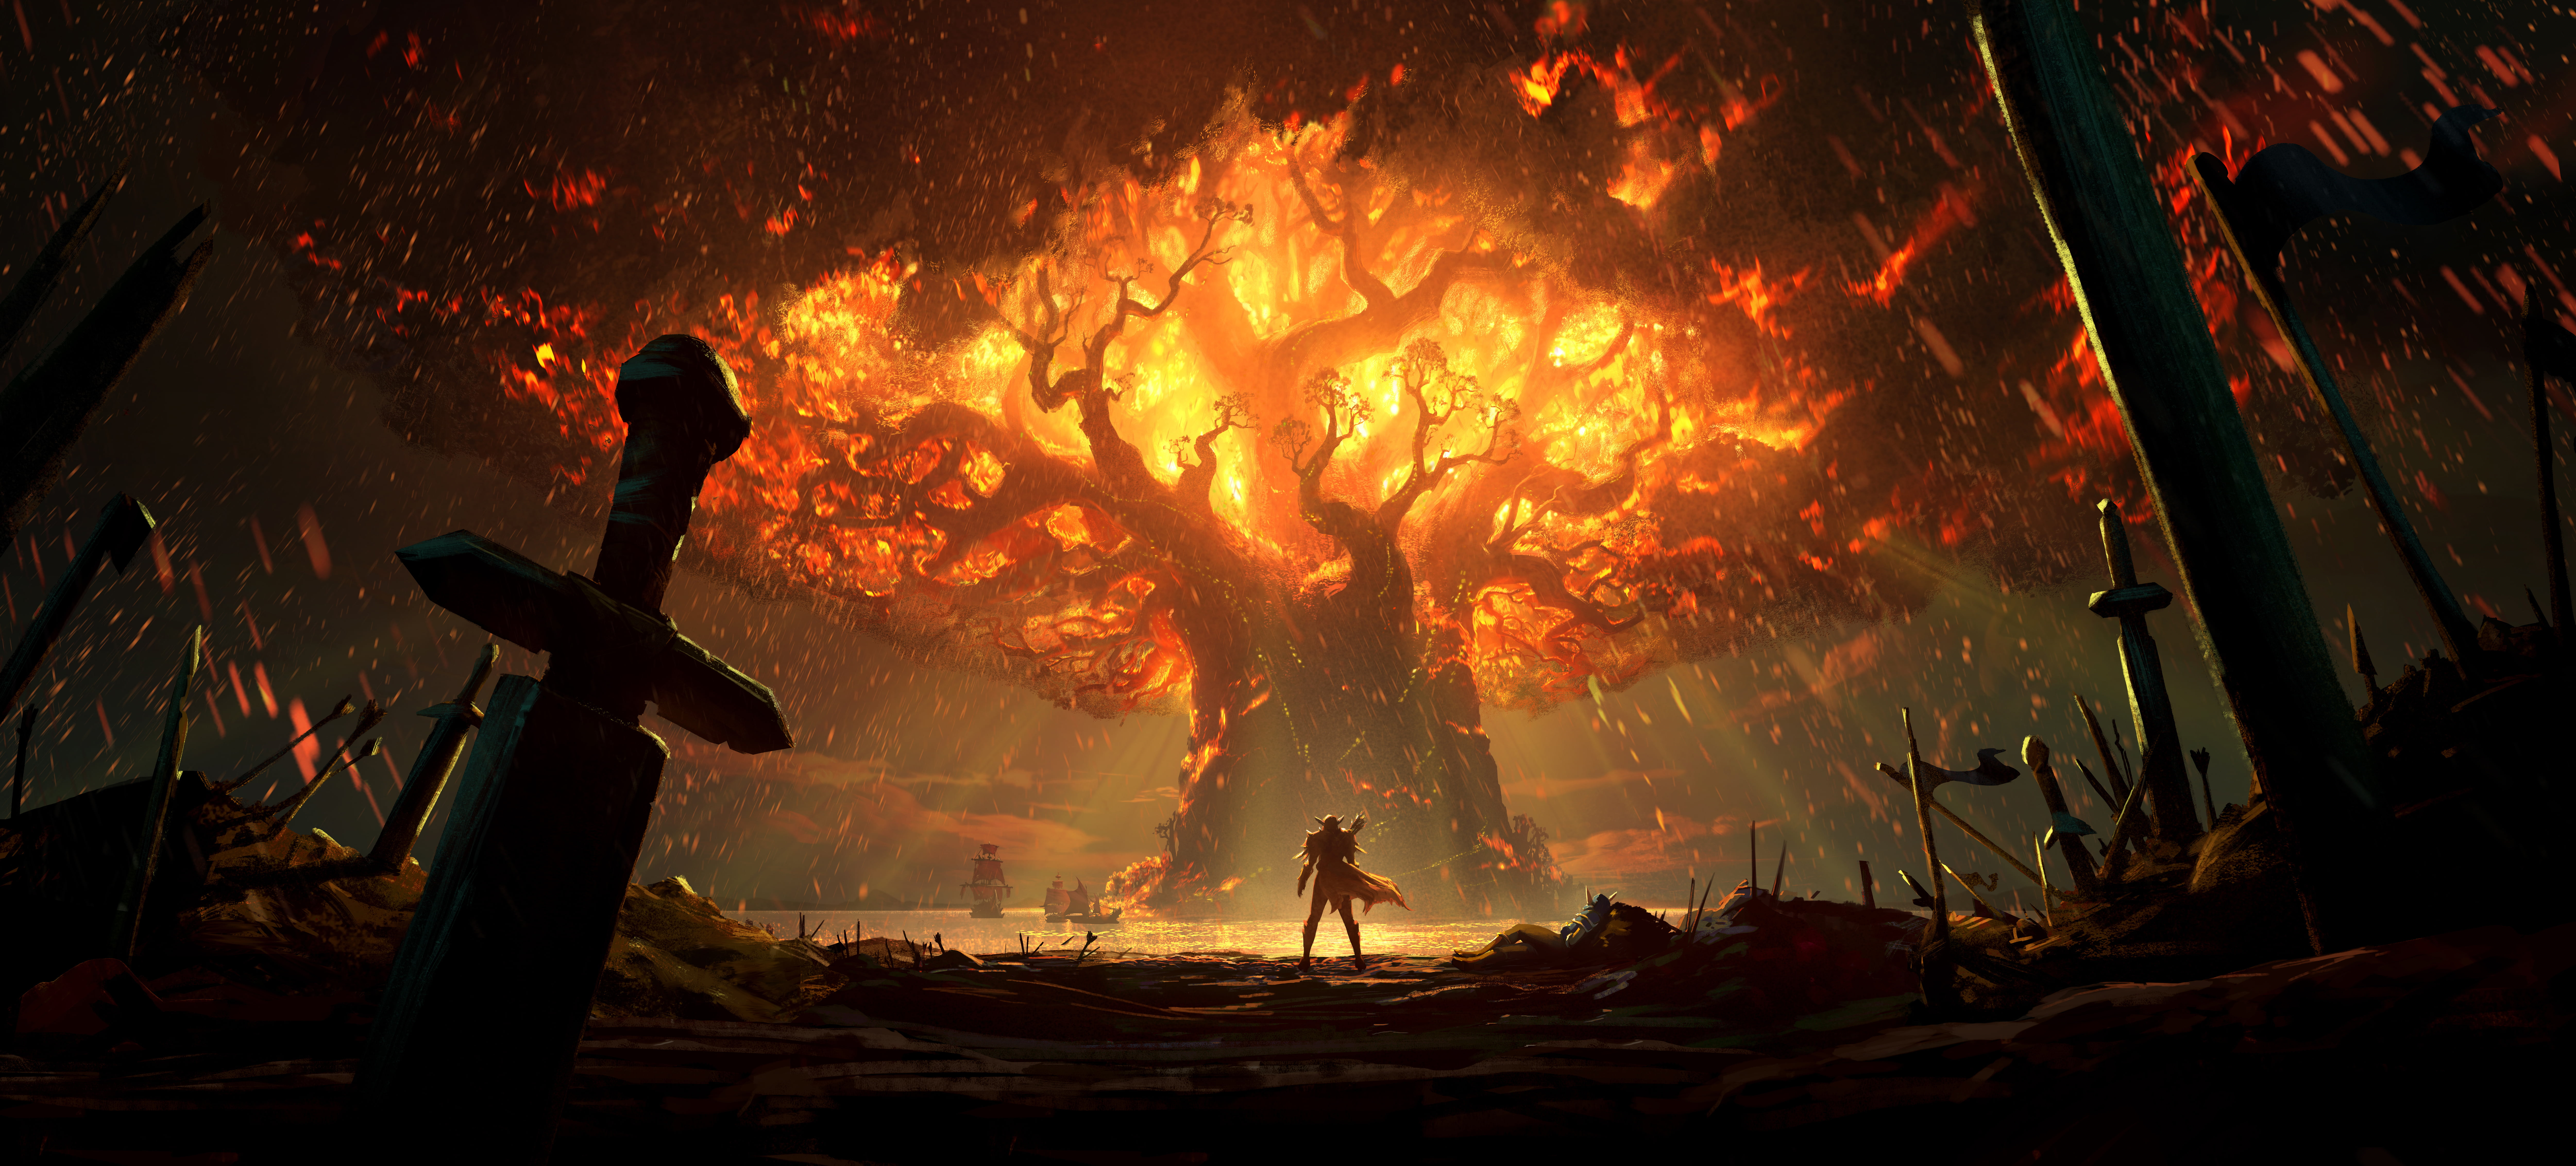
\includegraphics[scale=0.05]{images/wallpaperflare.com_wallpaper (1).jpg}
    image2:\newline
    \includegraphics[angle=90]{images/latex-tutorial.png}
    \newpage
    image3:\newline
    \includegraphics[width=\textwidth]{images/wallpaperflare.com_wallpaper (4).jpg}

    \subsection{figure environment}
    \begin{figure}[h]
        \centering
        \includegraphics[scale=0.04]{images/wallpaperflare.com_wallpaper (6).jpg}
        \caption{Plane}
        \label{fig:freedom}
    \end{figure}

    \subsection{table environment}
    \begin{table}[h]
        \centering
        \begin{tabular}{c c}
            \includegraphics[scale=0.05]{images/wallpaper.jpg} & \includegraphics[scale=0.05]{images/wallpaperflare.com_wallpaper (2).jpg} \\
            pic1 & pic2\\
        \end{tabular}
    \end{table}
    \section{Bibliography}
    \subsection{BibTeX}

    Compiler is the greatest invention of mankind. \cite{dragonbook}.\\
    MIPS is hard.
    \cite{mips}\\
    I am not a robot.
    \cite{turing2009computing}
    \bibliographystyle{plain}
    \bibliography{reference}
    
\end{document}